\chapter{Culling}
\label{sec:culling}

Culling is motivated by the fact, that \ac{BA} complexity grows with the number of \acp{KF} and that it enables lifelong operation in the same environment as the number of \acp{KF} will not grow unbounded \cite{Mur-Artal2015}.

ORB-SLAM2 \cite{Mur-Artal2016} already implemented a \ac{KF} culling mechanism which works locally. As the proposed new approach uses multiple \acp{KFM} to merge two maps, \ac{KF} culling within the merging procedure could remove redundant \acp{KF} from a bigger area compared to the standard \ac{KF} culling approach of ORB-SLAM2.

\section{Approach}

The culling of \acp{KF} is an additional step in the map merging procedure which is executed after $n$ \acp{KFM} were found and before the maps are aligned and the \acp{MP} fused.

The culling during the map merging follows the same approach as the one used for the local \ac{KF} culling in ORB-SLAM \cite{Mur-Artal2015}: All the \acp{KF} which observe a certain percentage of \acp{MP}, the redundancy threshold, which have also been seen in at least other three \acp{KF} in the same or finer scale, are discarded.

Culling of \acp{KF} is performed for every \ac{KFM} separately. Therefore the \acp{KF} which are considered for culling per \ac{KFM} are the two \acp{KF} of the \ac{KFM} and their direct neighbors in the co-visibility graph. \autoref{fig:culling0} visualizes this, where the \textcolor{blue}{blue ellipses} indicate the direct neighbors in the co-visibility graph and the \textcolor{red}{red ellipse} surrounds all the \acp{KF} which are considered for the culling for one \ac{KFM}.

\tikzstyle{abstract}=[rectangle, draw=black, rounded corners, fill=white!40, drop shadow,
        text centered, anchor=north, text=black, text width=3cm]
\begin{figure}[H]
  \centering
%  \begin{tikzpicture}[auto]
%    \node[entity] (key frame match) {\ac{KFM}}
%      [grow=down,sibling distance=4.5cm]
%        child {node[entity] (child 1) {\ac{KF}, map 1}
%          [grow=down,sibling distance=1.2cm]
%          child {node[entity,minimum size=1cm] {\ac{KF} 1}}
%          child {node[entity,minimum size=1cm] {\ac{KF} 2}}
%          child {node[entity,minimum size=1cm] {\ac{KF} $k$}}}
%        child {node[entity] {\ac{KF}, map 2}
%          [grow=down,sibling distance=1.2cm]
%          child {node[entity,minimum size=1cm] {\ac{KF} 1}}
%          child {node[entity,minimum size=1cm] {\ac{KF} 2}}
%          child {node[entity,minimum size=1cm] {\ac{KF} $l$}}};
%
%    \draw[blue,thick,dashed] (-2.25,-2.25) ellipse (1.5 and 0.5);
%
%    \draw[blue,thick,dashed] (2.25,-2.25) ellipse (1.5 and 0.5);
%
%    \draw[red,thick,dashed] (0,-2.25) ellipse (5 and 1.5);
%  \end{tikzpicture}

%  \begin{tikzpicture}[auto]
%  \node (KFM) [abstract, rectangle split, rectangle split parts=3]
%  {
%    \textbf{\ac{KFM}}
%    \nodepart{second}\ac{KF}, map 1
%    \nodepart{third}\ac{KF}, map 2
%  };
%  \end{tikzpicture}

  \begin{tikzpicture}
    % Box representing the KFM with two KFs
    \draw (-0.1, 1.9) -- (4.1, 1.9) -- (4.1, 4) -- (-0.1, 4) -- (-0.1, 1.9);
    \node at (2, 3.5)  {\ac{KFM}};
    \node[entity] at (1, 2.5) (kfm_kf1)  {\ac{KF}, map 1};
    \node[entity] at (3, 2.5) (kfm_kf2) {\ac{KF}, map 2};

    % Co-visibility graph kfs
    \node[entity,minimum width=1cm] at (-2.0, 0.75) (kf_1) {\ac{KF} 1};
    \node[entity,minimum width=1cm] at (-0.5, 0.75) (kf_2) {\ac{KF} 2};
    \node[entity,minimum width=1cm] at (1.0, 0.75) (kf_3) {\ac{KF} $k$};

    \node[entity,minimum width=1cm] at (6.0, 0.75) (kf_4) {\ac{KF} $l$};
    \node[entity,minimum width=1cm] at (4.5, 0.75) (kf_5) {\ac{KF} 2};
    \node[entity,minimum width=1cm] at (3.0, 0.75) (kf_6) {\ac{KF} 1};

    % Edges between kfm kfs and co-visibility graph kfs
    \draw (kfm_kf1.south) -- (kf_1.north);
    \draw (kfm_kf1.south) -- (kf_2.north);
    \draw (kfm_kf1.south) -- (kf_3.north);
    \draw (kfm_kf2.south) -- (kf_4.north);
    \draw (kfm_kf2.south) -- (kf_5.north);
    \draw (kfm_kf2.south) -- (kf_6.north);

    % Ellipses
    \draw[blue,thick,dashed] (-0.5, 1.625) ellipse (2.25 and 0.75);
    \draw[blue,thick,dashed] (4.5, 1.625) ellipse (2.25 and 0.75);
    \draw[red,thick,dashed] (2.0, 1.4) ellipse (5 and 1.75);
  \end{tikzpicture}
  \caption{\ac{KFM} with its \acp{KF} and their direct neighbors in the \textcolor{blue}{co-visibility graph}}
  \label{fig:culling0}
\end{figure}

To illustrate the culling procedure, \autoref{fig:culling1} shows the maps of two robots in a toy example.

\begin{figure}[H]
  \centering
  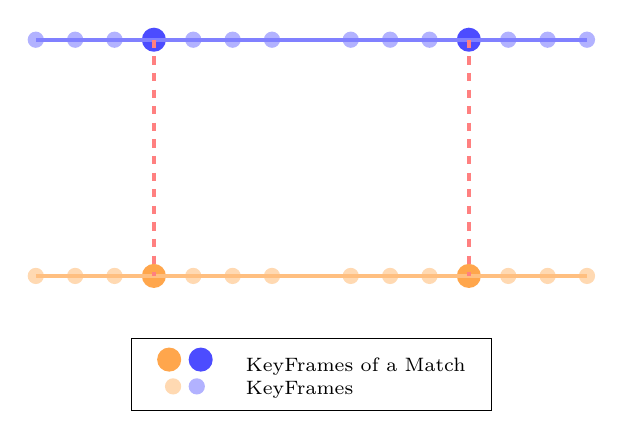
\begin{tikzpicture}[auto]
    \coordinate (A1) at (-0.5, 0);
    \coordinate (KFM11) at (1, 0);
    \coordinate (A1MP1) at (-0.5, 0);
    \coordinate (A1MP2) at (0, 0);
    \coordinate (A1MP3) at (0.5, 0);
    \coordinate (A1MP4) at (1.5, 0);
    \coordinate (A1MP5) at (2, 0);
    \coordinate (A1MP6) at (2.5, 0);

    \coordinate (B1) at (6.5, 0);
    \coordinate (KFM12) at (5, 0);
    \coordinate (B1MP1) at (5.5, 0);
    \coordinate (B1MP2) at (6.0, 0);
    \coordinate (B1MP3) at (6.5, 0);
    \coordinate (B1MP4) at (4.5, 0);
    \coordinate (B1MP5) at (4.0, 0);
    \coordinate (B1MP6) at (3.5, 0);

    \coordinate (A2) at (-0.5, -3);
    \coordinate (KFM21) at (1, -3);
    \coordinate (A2MP1) at (-0.5, -3);
    \coordinate (A2MP2) at (0, -3);
    \coordinate (A2MP3) at (0.5, -3);
    \coordinate (A2MP4) at (1.5, -3);
    \coordinate (A2MP5) at (2, -3);
    \coordinate (A2MP6) at (2.5, -3);

    \coordinate (B2) at (6.5, -3);
    \coordinate (KFM22) at (5, -3);
    \coordinate (B2MP1) at (5.5, -3);
    \coordinate (B2MP2) at (6.0, -3);
    \coordinate (B2MP3) at (6.5, -3);
    \coordinate (B2MP4) at (4.5, -3);
    \coordinate (B2MP5) at (4.0, -3);
    \coordinate (B2MP6) at (3.5, -3);

    \node [fill=blue!30, circle,inner sep=2pt, text width=0.1mm] at (A1MP1) {};
    \node [fill=blue!30, circle,inner sep=2pt, text width=0.1mm] at (A1MP2) {};
    \node [fill=blue!30, circle,inner sep=2pt, text width=0.1mm] at (A1MP3) {};
    \node [fill=blue!70, circle,inner sep=3pt, text width=0.1mm] at (KFM11) {};
    \node [fill=blue!30, circle,inner sep=2pt, text width=0.1mm] at (A1MP4) {};
    \node [fill=blue!30, circle,inner sep=2pt, text width=0.1mm] at (A1MP5) {};
    \node [fill=blue!30, circle,inner sep=2pt, text width=0.1mm] at (A1MP6) {};

    \node [fill=blue!30, circle,inner sep=2pt, text width=0.1mm] at (B1MP1) {};
    \node [fill=blue!30, circle,inner sep=2pt, text width=0.1mm] at (B1MP2) {};
    \node [fill=blue!30, circle,inner sep=2pt, text width=0.1mm] at (B1MP3) {};
    \node [fill=blue!70, circle,inner sep=3pt, text width=0.1mm] at (KFM12) {};
    \node [fill=blue!30, circle,inner sep=2pt, text width=0.1mm] at (B1MP4) {};
    \node [fill=blue!30, circle,inner sep=2pt, text width=0.1mm] at (B1MP5) {};
    \node [fill=blue!30, circle,inner sep=2pt, text width=0.1mm] at (B1MP6) {};

    \node [fill=orange!30, circle,inner sep=2pt, text width=0.1mm] at (A2MP1) {};
    \node [fill=orange!30, circle,inner sep=2pt, text width=0.1mm] at (A2MP2) {};
    \node [fill=orange!30, circle,inner sep=2pt, text width=0.1mm] at (A2MP3) {};
    \node [fill=orange!70, circle,inner sep=3pt, text width=0.1mm] at (KFM21) {};
    \node [fill=orange!30, circle,inner sep=2pt, text width=0.1mm] at (A2MP4) {};
    \node [fill=orange!30, circle,inner sep=2pt, text width=0.1mm] at (A2MP5) {};
    \node [fill=orange!30, circle,inner sep=2pt, text width=0.1mm] at (A2MP6) {};

    \node [fill=orange!30, circle,inner sep=2pt, text width=0.1mm] at (B2MP1) {};
    \node [fill=orange!30, circle,inner sep=2pt, text width=0.1mm] at (B2MP2) {};
    \node [fill=orange!30, circle,inner sep=2pt, text width=0.1mm] at (B2MP3) {};
    \node [fill=orange!70, circle,inner sep=3pt, text width=0.1mm] at (KFM22) {};
    \node [fill=orange!30, circle,inner sep=2pt, text width=0.1mm] at (B2MP4) {};
    \node [fill=orange!30, circle,inner sep=2pt, text width=0.1mm] at (B2MP5) {};
    \node [fill=orange!30, circle,inner sep=2pt, text width=0.1mm] at (B2MP6) {};

    \draw [blue!50, line width=0.05cm] (A1) to (B1);
    \draw [orange!50, line width=0.05cm] (A2) to (B2);

    \draw [red!50, line width=0.05cm, dashed] (KFM11) to (KFM21);
    \draw [red!50, line width=0.05cm, dashed] (KFM12) to (KFM22);

    \node[draw] at (3.0, -4.25)
    {
    \scriptsize
    \begin{tabular}{cl}
      \tikz\node[fill=orange!70, circle,inner sep=3pt, text width=0.1mm] {}; \tikz\node[fill=blue!70, circle,inner sep=3pt, text width=0.1mm] {}; & KeyFrames of a Match \\
      \tikz\node[fill=orange!30, circle,inner sep=2.0pt, text width=0.1mm] {}; \tikz\node[fill=blue!30, circle,inner sep=2.0pt, text width=0.1mm] {}; & KeyFrames \\
    \end{tabular}
    };
    \end{tikzpicture}
  \caption{Toy example of the map of two clients}
  \label{fig:culling1}
\end{figure}

\autoref{fig:culling2} then shows the \acp{KF} which are directly connected to the \acp{KF} of a \ac{KFM} indicated by dashed rectangles.

\begin{figure}[H]
  \centering
  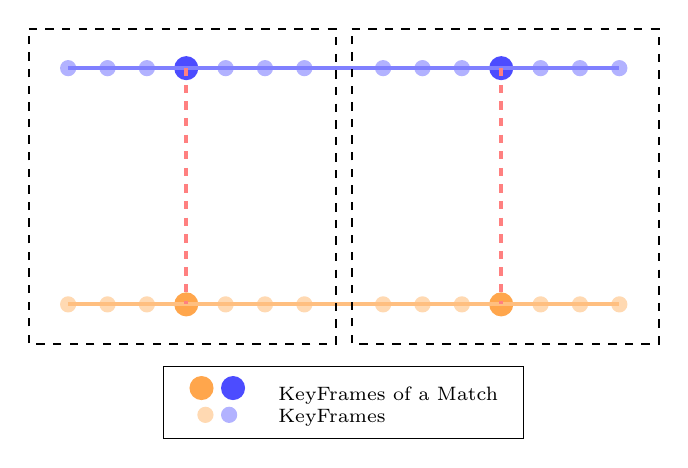
\begin{tikzpicture}[auto]
    \coordinate (A1) at (-0.5, 0);
    \coordinate (KFM11) at (1, 0);
    \coordinate (A1MP1) at (-0.5, 0);
    \coordinate (A1MP2) at (0, 0);
    \coordinate (A1MP3) at (0.5, 0);
    \coordinate (A1MP4) at (1.5, 0);
    \coordinate (A1MP5) at (2, 0);
    \coordinate (A1MP6) at (2.5, 0);

    \coordinate (B1) at (6.5, 0);
    \coordinate (KFM12) at (5, 0);
    \coordinate (B1MP1) at (5.5, 0);
    \coordinate (B1MP2) at (6.0, 0);
    \coordinate (B1MP3) at (6.5, 0);
    \coordinate (B1MP4) at (4.5, 0);
    \coordinate (B1MP5) at (4.0, 0);
    \coordinate (B1MP6) at (3.5, 0);

    \coordinate (A2) at (-0.5, -3);
    \coordinate (KFM21) at (1, -3);
    \coordinate (A2MP1) at (-0.5, -3);
    \coordinate (A2MP2) at (0, -3);
    \coordinate (A2MP3) at (0.5, -3);
    \coordinate (A2MP4) at (1.5, -3);
    \coordinate (A2MP5) at (2, -3);
    \coordinate (A2MP6) at (2.5, -3);

    \coordinate (B2) at (6.5, -3);
    \coordinate (KFM22) at (5, -3);
    \coordinate (B2MP1) at (5.5, -3);
    \coordinate (B2MP2) at (6.0, -3);
    \coordinate (B2MP3) at (6.5, -3);
    \coordinate (B2MP4) at (4.5, -3);
    \coordinate (B2MP5) at (4.0, -3);
    \coordinate (B2MP6) at (3.5, -3);

    \node [fill=blue!30, circle,inner sep=2pt, text width=0.1mm] at (A1MP1) {};
    \node [fill=blue!30, circle,inner sep=2pt, text width=0.1mm] at (A1MP2) {};
    \node [fill=blue!30, circle,inner sep=2pt, text width=0.1mm] at (A1MP3) {};
    \node [fill=blue!70, circle,inner sep=3pt, text width=0.1mm] at (KFM11) {};
    \node [fill=blue!30, circle,inner sep=2pt, text width=0.1mm] at (A1MP4) {};
    \node [fill=blue!30, circle,inner sep=2pt, text width=0.1mm] at (A1MP5) {};
    \node [fill=blue!30, circle,inner sep=2pt, text width=0.1mm] at (A1MP6) {};

    \node [fill=blue!30, circle,inner sep=2pt, text width=0.1mm] at (B1MP1) {};
    \node [fill=blue!30, circle,inner sep=2pt, text width=0.1mm] at (B1MP2) {};
    \node [fill=blue!30, circle,inner sep=2pt, text width=0.1mm] at (B1MP3) {};
    \node [fill=blue!70, circle,inner sep=3pt, text width=0.1mm] at (KFM12) {};
    \node [fill=blue!30, circle,inner sep=2pt, text width=0.1mm] at (B1MP4) {};
    \node [fill=blue!30, circle,inner sep=2pt, text width=0.1mm] at (B1MP5) {};
    \node [fill=blue!30, circle,inner sep=2pt, text width=0.1mm] at (B1MP6) {};

    \node [fill=orange!30, circle,inner sep=2pt, text width=0.1mm] at (A2MP1) {};
    \node [fill=orange!30, circle,inner sep=2pt, text width=0.1mm] at (A2MP2) {};
    \node [fill=orange!30, circle,inner sep=2pt, text width=0.1mm] at (A2MP3) {};
    \node [fill=orange!70, circle,inner sep=3pt, text width=0.1mm] at (KFM21) {};
    \node [fill=orange!30, circle,inner sep=2pt, text width=0.1mm] at (A2MP4) {};
    \node [fill=orange!30, circle,inner sep=2pt, text width=0.1mm] at (A2MP5) {};
    \node [fill=orange!30, circle,inner sep=2pt, text width=0.1mm] at (A2MP6) {};

    \node [fill=orange!30, circle,inner sep=2pt, text width=0.1mm] at (B2MP1) {};
    \node [fill=orange!30, circle,inner sep=2pt, text width=0.1mm] at (B2MP2) {};
    \node [fill=orange!30, circle,inner sep=2pt, text width=0.1mm] at (B2MP3) {};
    \node [fill=orange!70, circle,inner sep=3pt, text width=0.1mm] at (KFM22) {};
    \node [fill=orange!30, circle,inner sep=2pt, text width=0.1mm] at (B2MP4) {};
    \node [fill=orange!30, circle,inner sep=2pt, text width=0.1mm] at (B2MP5) {};
    \node [fill=orange!30, circle,inner sep=2pt, text width=0.1mm] at (B2MP6) {};

    \draw [blue!50, line width=0.05cm] (A1) to (B1);
    \draw [orange!50, line width=0.05cm] (A2) to (B2);

    \draw [red!50, line width=0.05cm, dashed] (KFM11) to (KFM21);
    \draw [red!50, line width=0.05cm, dashed] (KFM12) to (KFM22);

    \draw[black,thick,dashed] (-1, 0.5) -- (2.9, 0.5) -- (2.9, -3.5) -- (-1, -3.5) -- (-1, 0.5);
    \draw[black,thick,dashed] (3.1, 0.5) -- (7.0, 0.5) -- (7.0, -3.5) -- (3.1, -3.5) -- (3.1, 0.5);

    \node[draw] at (3.0, -4.25)
    {
    \scriptsize
    \begin{tabular}{cl}
      \tikz\node[fill=orange!70, circle,inner sep=3pt, text width=0.1mm] {}; \tikz\node[fill=blue!70, circle,inner sep=3pt, text width=0.1mm] {}; & KeyFrames of a Match \\
      \tikz\node[fill=orange!30, circle,inner sep=2.0pt, text width=0.1mm] {}; \tikz\node[fill=blue!30, circle,inner sep=2.0pt, text width=0.1mm] {}; & KeyFrames \\
    \end{tabular}
    };
    \end{tikzpicture}
  \caption{Two \acp{KFM} with their neighborhood}
  \label{fig:culling2}
\end{figure}

The toy example with culled \acp{KF} is shown in \autoref{fig:culling3}, where the \textcolor{red}{x} represent culled \acp{KF}.

\begin{figure}[H]
  \centering
  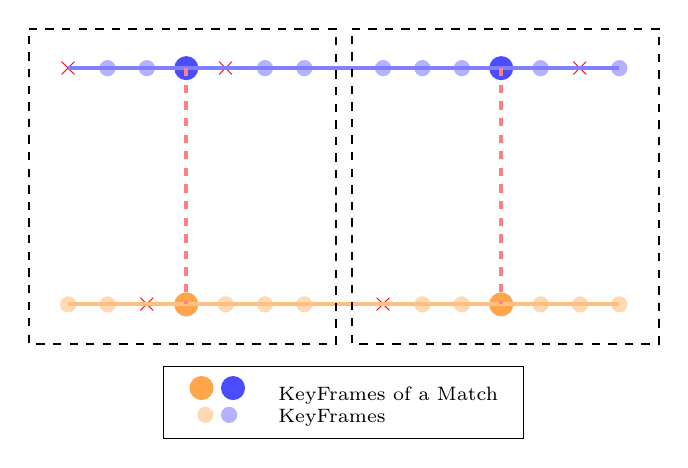
\begin{tikzpicture}[auto]
    \coordinate (A1) at (-0.5, 0);
    \coordinate (KFM11) at (1, 0);
    \coordinate (A1MP1) at (-0.5, 0);
    \coordinate (A1MP2) at (0, 0);
    \coordinate (A1MP3) at (0.5, 0);
    \coordinate (A1MP4) at (1.5, 0);
    \coordinate (A1MP5) at (2, 0);
    \coordinate (A1MP6) at (2.5, 0);

    \coordinate (B1) at (6.5, 0);
    \coordinate (KFM12) at (5, 0);
    \coordinate (B1MP1) at (5.5, 0);
    \coordinate (B1MP2) at (6.0, 0);
    \coordinate (B1MP3) at (6.5, 0);
    \coordinate (B1MP4) at (4.5, 0);
    \coordinate (B1MP5) at (4.0, 0);
    \coordinate (B1MP6) at (3.5, 0);

    \coordinate (A2) at (-0.5, -3);
    \coordinate (KFM21) at (1, -3);
    \coordinate (A2MP1) at (-0.5, -3);
    \coordinate (A2MP2) at (0, -3);
    \coordinate (A2MP3) at (0.5, -3);
    \coordinate (A2MP4) at (1.5, -3);
    \coordinate (A2MP5) at (2, -3);
    \coordinate (A2MP6) at (2.5, -3);

    \coordinate (B2) at (6.5, -3);
    \coordinate (KFM22) at (5, -3);
    \coordinate (B2MP1) at (5.5, -3);
    \coordinate (B2MP2) at (6.0, -3);
    \coordinate (B2MP3) at (6.5, -3);
    \coordinate (B2MP4) at (4.5, -3);
    \coordinate (B2MP5) at (4.0, -3);
    \coordinate (B2MP6) at (3.5, -3);

    \node [red] at (A1MP1) {$\boldsymbol{\times}$};
    \node [fill=blue!30, circle,inner sep=2pt, text width=0.1mm] at (A1MP2) {};
    \node [fill=blue!30, circle,inner sep=2pt, text width=0.1mm] at (A1MP3) {};
    \node [fill=blue!70, circle,inner sep=3pt, text width=0.1mm] at (KFM11) {};
    \node [red] at (A1MP4) {$\boldsymbol{\times}$};
    \node [fill=blue!30, circle,inner sep=2pt, text width=0.1mm] at (A1MP5) {};
    \node [fill=blue!30, circle,inner sep=2pt, text width=0.1mm] at (A1MP6) {};

    \node [fill=blue!30, circle,inner sep=2pt, text width=0.1mm] at (B1MP1) {};
    \node [red] at (B1MP2) {$\boldsymbol{\times}$};
    \node [fill=blue!30, circle,inner sep=2pt, text width=0.1mm] at (B1MP3) {};
    \node [fill=blue!70, circle,inner sep=3pt, text width=0.1mm] at (KFM12) {};
    \node [fill=blue!30, circle,inner sep=2pt, text width=0.1mm] at (B1MP4) {};
    \node [fill=blue!30, circle,inner sep=2pt, text width=0.1mm] at (B1MP5) {};
    \node [fill=blue!30, circle,inner sep=2pt, text width=0.1mm] at (B1MP6) {};

    \node [fill=orange!30, circle,inner sep=2pt, text width=0.1mm] at (A2MP1) {};
    \node [fill=orange!30, circle,inner sep=2pt, text width=0.1mm] at (A2MP2) {};
    \node [red] at (A2MP3) {$\boldsymbol{\times}$};
    \node [fill=orange!70, circle,inner sep=3pt, text width=0.1mm] at (KFM21) {};
    \node [fill=orange!30, circle,inner sep=2pt, text width=0.1mm] at (A2MP4) {};
    \node [fill=orange!30, circle,inner sep=2pt, text width=0.1mm] at (A2MP5) {};
    \node [fill=orange!30, circle,inner sep=2pt, text width=0.1mm] at (A2MP6) {};

    \node [fill=orange!30, circle,inner sep=2pt, text width=0.1mm] at (B2MP1) {};
    \node [fill=orange!30, circle,inner sep=2pt, text width=0.1mm] at (B2MP2) {};
    \node [fill=orange!30, circle,inner sep=2pt, text width=0.1mm] at (B2MP3) {};
    \node [fill=orange!70, circle,inner sep=3pt, text width=0.1mm] at (KFM22) {};
    \node [fill=orange!30, circle,inner sep=2pt, text width=0.1mm] at (B2MP4) {};
    \node [fill=orange!30, circle,inner sep=2pt, text width=0.1mm] at (B2MP5) {};
    \node [red] at (B2MP6) {$\boldsymbol{\times}$};

    \draw [blue!50, line width=0.05cm] (A1) to (B1);
    \draw [orange!50, line width=0.05cm] (A2) to (B2);

    \draw [red!50, line width=0.05cm, dashed] (KFM11) to (KFM21);
    \draw [red!50, line width=0.05cm, dashed] (KFM12) to (KFM22);

    \draw[black,thick,dashed] (-1, 0.5) -- (2.9, 0.5) -- (2.9, -3.5) -- (-1, -3.5) -- (-1, 0.5);
    \draw[black,thick,dashed] (3.1, 0.5) -- (7.0, 0.5) -- (7.0, -3.5) -- (3.1, -3.5) -- (3.1, 0.5);

    \node[draw] at (3.0, -4.25)
    {
    \scriptsize
    \begin{tabular}{cl}
      \tikz\node[fill=orange!70, circle,inner sep=3pt, text width=0.1mm] {}; \tikz\node[fill=blue!70, circle,inner sep=3pt, text width=0.1mm] {}; & KeyFrames of a Match \\
      \tikz\node[fill=orange!30, circle,inner sep=2.0pt, text width=0.1mm] {}; \tikz\node[fill=blue!30, circle,inner sep=2.0pt, text width=0.1mm] {}; & KeyFrames \\
    \end{tabular}
    };
    \end{tikzpicture}
  \caption{\acp{KF} culled}
  \label{fig:culling3}
\end{figure}
